\section{Background on application}\label{back}
The application receives the ZIP file with images to be resized and also custom user parameters, if specified. Images in JPG and PNG format are supported. The application then extracts the images and resizes them to 4 different sizes. These resized images are then put into another ZIP file and sent back to the user. The image processing itself is performed on slave virtual machines, which are chosen by master machine according to their CPU load.

\subsection{Application requirements}
WantCloud requires the application to fulfil basic requirements laid on all cloud computing applications. In particular, it means that application should satisfy these requirements:

The system should...
\begin{enumerate}
 \item automatically decide whether it should start more Virtual Machines and the incoming jobs should be automatically distributed among these machines.
 \item offer such functionalities to start and stop rented machines.
 \item allocate new jobs to the least utilized machines.
 \item offer policies for sudden system failures.
 \item keep usage statistics and performance metrics.
\end{enumerate}

\section{System Design}\label{sysdesign}
%Background on Application (recommended size: 0.5 pages): describe the application (1
%paragraph) and its requirements (1-3 paragraphs, summarized in a table if needed).
%5. System Design (recommended size: 1.5 pages)
%a. Resource Management Architecture: describe the design of your system,
%including the inter-operation of the provisioning, allocation, reliability, and
%monitoring components (which correspond to the homonym features required
%by the WantCloud CTO).
%b. System Policies: describe the policies your system uses and supports. The latter
%may remain not implemented throughout your coursework, as long as you can
%explain how they can be supported in the future.
%c. (Optional, for bonus points, see Section F) Additional System Features:
%describe each additional feature of your system, one sub-section per feature.
\subsection{Overview}
The application is designed as a typical client/server application. Client can specify in CLI\footnote{Command line} parameters which file to upload and what sizes of images to request. The client first contacts the master server, which will send the user the address of a slave machine, which will process the job. The client then automatically uploads the file to the slave machine, where it is processed and sent back to the client.

The master instance of the server consists of these main parts:

\begin{enumerate}
 \item \emph{Listener}. Listens to clients through TCP socket, when a client connects, it asks VM Manager for the least utilized slave Virtual Machine and returns its address to the client.
 \item \emph{VM Manager}. This component is responsible for provisioning slave instances. When a utilization of a machine is bellow certain threshold, this machine is stopped. On the other hand, when a machine is highly utilized and other machines are available, one of them is started.
 \item \emph{Monitor}. Monitor communicates via TCP socket with slave machines and updates information about their performance, so their utilization can be easily resolved.
\end{enumerate}

Slave instances of the server are composed of these main parts:

\begin{enumerate}
 \item \emph{Connection Handler}. This component is responsible for accepting ZIP file from the clients and sending ZIP files with resized images back to them.
 \item \emph{Job Processor}. Main component responsible for image processing itself. It unpacks the ZIP file, resizes images to all 4 different sizes and creates new ZIP from them.
 \item \emph{Monitor}. Monitor collects the information about usage of the machine and its performance. It also generates log reports and sends these information to master Monitor.
\end{enumerate}

You can see the design of the application on figure \ref{architecture}. Solid lines represent a lifespan of a submitted job, dashed lines then represent asynchronous operations, which are regularly started on the server. 

\begin{figure}
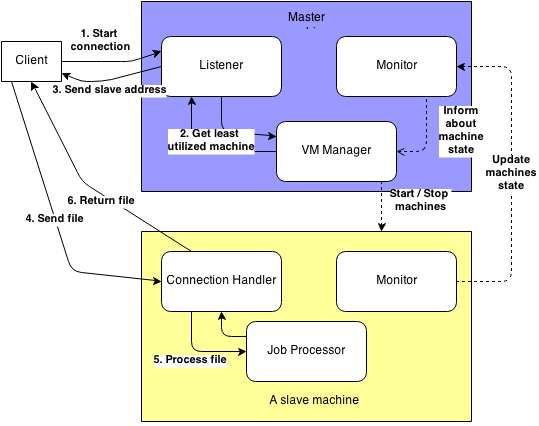
\includegraphics[scale=0.5]{architecture}
\label{architecture}
\caption{Overview of system architecture}
\end{figure}


\subsection{Resource Management Architecture}

In this section we will describe several system features to give a better insight into the whole resource management architecture.

\subsubsection{Master Virtual Machine}
Master Virtual Machine is responsible for managing slave Virtual Machines and pointing incoming clients to these machines. The master server is running three main threads:
\begin{itemize}
 \item Listener thread, which is responsible for accepting clients and pointing them to the right slave machine.
 \item VM Manager thread, which constantly leverages Virtual Machine information received from the Monitor to watch over the state of Virtual Machines and which decides whether they should be started, stopped or kept running.
 \item Monitor thread, which receives and stores information about performance from the slave machines and informs the VM Manager about this.
\end{itemize}

The address of the master server is the only address, which the client requires to know. Addresses of slave machines responsible for image processing itself are dynamically sent to the client.

\subsubsection{Slave Virtual Machines}
Slave Virtual Machines are performing the image processing itself. After the client receives the address of a slave machine, it starts uploading ZIP file with images to process. After the upload, the ZIP file is given to the queue, from where the Job Processor starts resizing the images. There is a single thread for each job and therefore a slave machine can process multiple jobs simultaneously. However, a maximum number of jobs could be set in the future. %TODO implement and maybe experiment???
After the resizing, the images are put into new ZIP file, which is sent back via socket connection to the user.

Each slave machine is running three main threads:
\begin{itemize}
 \item Connection thread, which receives the ZIP file from the client, puts it to the queue and after the completion sends the ZIP file back.
 \item Job Processor thread, which dequeues the jobs from the queue and processes them.
 \item Monitor thread, which monitors system state and performance every second and regularly sends these information to master server. The thread is also responsible for logs generation.
\end{itemize}

\subsubsection{Summary}
This resource management architecture, as mentioned above, suffices all requirements:
\begin{enumerate}
 \item The system is fully automated, the client only needs to specify file to be processed. System will automatically decide on which machine the job should be processed and it will start and stop virtual machines to achieve more efficient utilization.
 \item The system is able to start and stop Amazon micro machines, according to the given policies.
 \item The system is able to schedule client on different slave machines, according to the given policies.
 \item In case of a failure of a machine a new machine will be started and the job can be restarted on this machine.
 \item System keeps track of its usage (number of users) and performance (CPU and Memory utilization) in the logs.
\end{enumerate}

\subsection{System policies}
\subsubsection{Allocation policies}
The job is allocated to the machine with lowest CPU utilization at the current moment. However, the system offers methods accessing other usage and performance metrics, which allows easy modification of this policy in the future.
\subsubsection{Provisioning policies}
New machines are provisioned when the normalized load is above a certain threshold. This normalized load is calculated by taking the CPU load of every machine and dividing it by the number of machines, it does the same for the memory load. Both loads are measured in percentage, in the range of 0-100. If one of the loads is above 75\%, the system will provision one new machine. Otherwise if both loads are under 35\%, it will send a signal to stop the machine with the lowest load. It will first let it finish its current task if it has one and then actually stop the machine. The threshold value can easily be tweaked in order to optimize performance, however, we leave this to future work.
\subsection{Implementation}
The system is implemented in Java and it leverages the following libraries:
\begin{itemize}
 \item JCommander\cite{jcommander} for easier parsing of parameters.
 \item Java Secure Channel\cite{jsch} for establishing SSH connection between master and slave machines.
 \item Sigar\cite{sigar} for getting the access to performance data.
 \item Amazon AWS SDK for Java\cite{aws}, to manage instances from Amazon Elastic Cloud Computing.
 \item ZIP Directory\cite{zip} for creating new ZIP from a folder.
\end{itemize}

\subsection{Multi Tenancy \emph{Additional System Feature}}
Through our client-server model we can serve a number of connecting clients on one slave machine. Through our elasticity we start multiple machines, thus we can expand the number of clients that can connect to our application. The bottleneck here, is the master machine which services the client requests, we could upgrade the machine itself to a better Amazon instance type to service more users if the need arises. 

Each user gets a fair share of the resources up to a maximum of one machine per user. If our number of machines gets depleted, new jobs will be put in a queue that will have to wait to be served. 